% 来源：OEBPS/Text/Section0001_split_006.xhtml#sigil_toc_id_46

\BookChapter{33}
\section[第33章\q 戴维·斯文森：管理239亿美元的工作都是爱]{第33章\\ 戴维·斯文森：管理239亿美元的工作都是爱}

\begin{figure}[htbp]
\centering
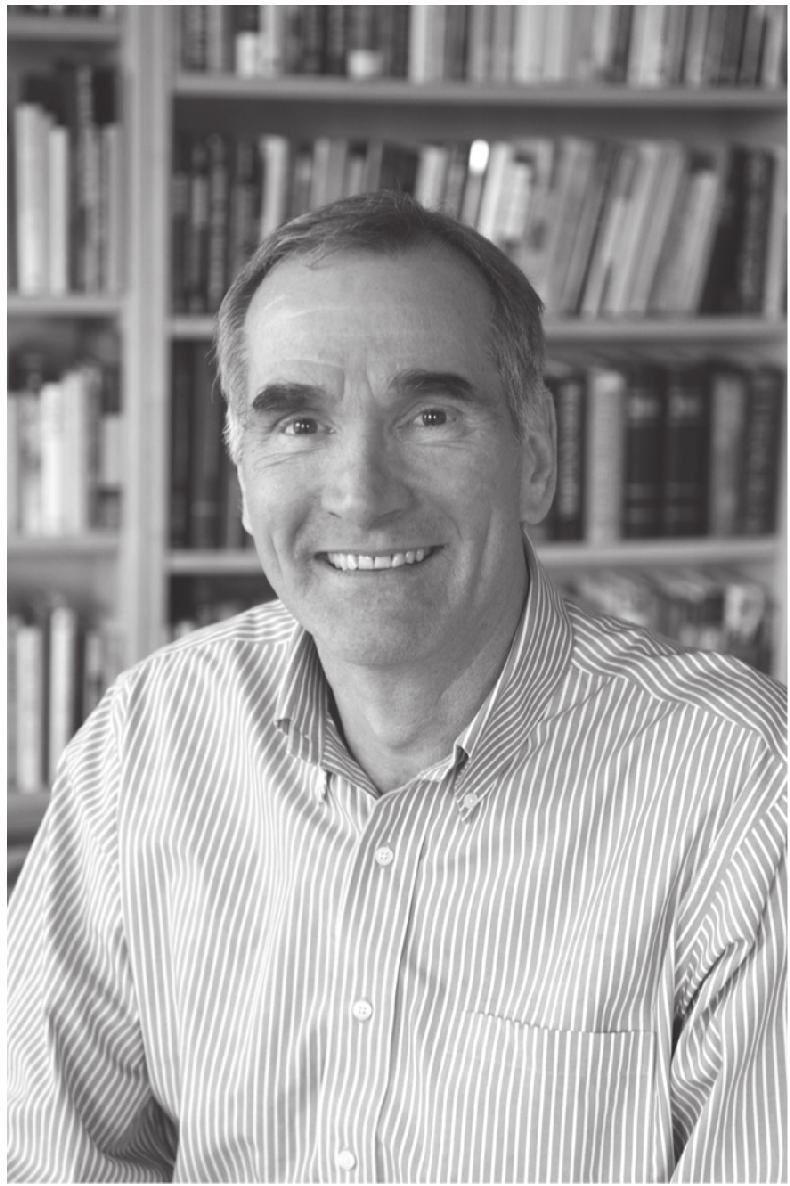
\includegraphics[width=0.40\linewidth,keepaspectratio]{image/戴维·斯文森肖像.jpg}
\caption*{戴维·斯文森}
\end{figure}

耶鲁大学首席投资官，著有《不落俗套的成功》

戴维·斯文森可能是你没有听说过的最有名的投资大师。有人称他为机构投资界的沃伦·巴菲特。戴维·斯文森担任耶鲁大学首席投资官27年，其间他把10亿美元的资产变成239亿美元，27年的年化收益率达到13.9\%，即使很多很牛的对冲基金业绩也无法与之相比，难怪在这27年中很多对冲基金一直在引诱他离开耶鲁大学，加入对冲基金肯定能让他的个人收入多上好几倍。

你要是见到斯文森，就会马上认识到他做这份工作不是为了钱，而是因为热爱投资这种比赛，还有那种服务一所伟大的大学的感觉。戴维·斯文森愿意一直领着耶鲁大学给的这份薪水，就证明这一点。他要是加入对冲基金，会让他的个人财富超过他在耶鲁大学收入的N多倍。

但是从核心原则来看，戴维·斯文森是发明者，也是毁灭者。戴维·斯文森的耶鲁大学投资模式，也被大家称为捐赠基金投资模式，是他和同事也是他以前的塔卡哈什教务长一起开发形成的，是现代投资组合理论的实践应用。这个投资模式就是把投资组合分成5\textasciitilde{}6个大致相等的部分，分别投资不同的资产类型。耶鲁大学投资模式是一个长期投资策略，喜欢范围非常宽广的分散投资，偏好股权投资，而不太强调投资收益较低的资产类型，比如债券或者大宗商品。业内也称戴维·斯文森在流动性上的立场是革命性的：他不追逐流动性，而且避开流动性，他的理由是流动性会导致收益率降低，如果不追逐流动性的话，这些资产可以投资得更有效率。

在他成为机构投资界的摇滚明星之前，戴维·斯文森在华尔街工作，就职于投资界的黄埔军校所罗门兄弟公司。很多人认为是戴维·斯文森设计出来全世界第一例货币掉期交易，那是IBM公司和世界银行之间的交易，事实上这导致了利率掉期以及最终的违约信贷掉期市场的产生，现在有1万亿美元的资产规模。不要因为这导致了金融危机而记恨于他！

我很荣幸能有机会和戴维·斯文森面对面地交谈。来到耶鲁大学，走进他的办公室，进入传说中的机构投资圣殿，我有些紧张。在此之前，我做了很多功课，任何一个好学生准备考试之前都会拼命复习，我也是通宵达旦地拼命恶补。我可不想让他看出来我有任何一点的准备不足，为此我仔细阅读了他写的那本400多页厚的书《不落俗套的成功》，他在书中讲的是关于个人投资和分散投资的观点。直到做完所有这些功课之后，我才满怀崇敬之心地去拜见这位资产配置大师。我们的访谈时间接近4个小时，下面是经过编辑的访谈内容的精简版本。

\begin{BookQuote}
\textbf{罗宾斯：}你为美国资产规模最大的机构之一工作，但是你非常关心个人投资者，花了很多时间精力为个人投资者提供指导，你为什么会这样做？请谈谈你的想法。
\end{BookQuote}

\begin{BookQuote}
\textbf{戴维·斯文森：}我基本上是一个乐观的人，但是一看到个人投资者面对的这个世界，真是一团糟，我很悲观。
\end{BookQuote}

\begin{BookQuote}
\textbf{罗宾斯：}为什么会这样？
\end{BookQuote}

\begin{BookQuote}
\textbf{戴维·斯文森：}投资者本来该有一些类型的投资选择，可事实上他们却没有，最根本的原因是公募基金行业以利润为导向。不要误解我的意思，我信奉市场经济，我相信做生意的目的就是赚取利润，但是在盈利动机和受托责任之间存在着一个基本的冲突，因为服务提供者的利润越高，投资者得到的收益就越低。
\end{BookQuote}

\begin{BookQuote}
\textbf{罗宾斯：}你说的受托责任，并不是所有的投资者都知道它是什么意思。我们真正能讨论的是：你必须把投资者的利益放在你自己的利益前面，以投资者利益为先，以投资者利益为重。
\end{BookQuote}

\begin{BookQuote}
\textbf{戴维·斯文森：}问题是公募基金公司积累的资产规模更大，收取的费用更高，自然赚的钱更多了。而高费用与投资人创造高收益的目标直接冲突。所以一次又一次发生的情况是，盈利赢了，寻找收益的投资者输了。现在有两个机构，这种利益冲突是不存在的，它们是先锋公司和美国教师退休金协会。这两个机构都是在非营利基础上经营的，它们寻求的是满足投资者的利益，所以它们是强大的受托人。在这两个机构里，受托责任最后总会赢。
\end{BookQuote}

\begin{BookQuote}
\textbf{罗宾斯：}因为公募基金业绩大部分都跑输市场。我读到过一篇文章，里面写道，1984—1998年，只有4\%的公募基金管理（规模超过1亿美元）战胜了先锋标准普尔500指数基金。但是这4\%的公募基金，每年都不一样。用更简单的话说就是，所有公募基金中有96\%的基金没能战胜市场。
\end{BookQuote}

\begin{BookQuote}
\textbf{戴维·斯文森：}那些统计数据只是冰山的一角。现实更加糟糕。你看过去的基金业绩的时候，只能看到至今还存在的基金的业绩。
\end{BookQuote}

\begin{BookQuote}
\textbf{罗宾斯：}只能看到幸存者，清算消失的基金就看不到历史业绩了。
\end{BookQuote}

\begin{BookQuote}
\textbf{戴维·斯文森：}你说得很对。这些统计数据都有幸存者偏差，过去10年里有好几百个公募基金都关掉了，再也看不到了，因为它们的业绩太差。当然，公募基金公司不会把那些业绩非常棒的基金合并到业绩非常差的基金里，它们肯定是反过来做的，把那些业绩非常糟糕的基金合并到业绩非常出色的基金里面，好基金并吞烂基金，这样公募基金公司里面就没有烂基金了，全都是好基金。
\end{BookQuote}

\begin{BookQuote}
\textbf{罗宾斯：}所以，统计数据说96\%的基金没有能够战胜市场，并不准确？
\end{BookQuote}

\begin{BookQuote}
\textbf{戴维·斯文森：}事实上更加糟糕，输给市场的公募基金超过96\%。
\end{BookQuote}

\begin{BookQuote}
\textbf{罗宾斯：}噢！
\end{BookQuote}

\begin{BookQuote}
\textbf{戴维·斯文森：}另一个原因表明，基金投资者真正得到的实际业绩，比你所引用的数据更加糟糕，这是因为我们作为个人投资者，自己的投资行为会有一些错误。个人投资者倾向于购买那些有良好业绩的基金，他们追逐收益。后来在基金业绩表现糟糕的时候，他们就会卖出。所以他们最终是高位买入低位卖出。要用这种方式赚钱，那就糟了。
\end{BookQuote}

\begin{BookQuote}
\textbf{罗宾斯：}追逐业绩的真实情况是什么？
\end{BookQuote}

\begin{BookQuote}
\textbf{戴维·斯文森：}这种事很多都跟市场营销有关。没有人愿意出去说：“我持有几只一星评级和二星评级的基金。”人们都想要持有四星评级的基金，还有五星评级的基金，然后在办公室里到处炫耀。
\end{BookQuote}

\begin{BookQuote}
\textbf{罗宾斯：}人之常情。
\end{BookQuote}

\begin{BookQuote}
\textbf{戴维·斯文森：}但是这些获得了四星和五星评级的基金，是那些过去业绩表现良好的基金，并不一定是那些将来业绩会表现良好的基金。如果你一直买的是那些过去业绩表现良好的基金，而卖出那些过去业绩表现糟糕的基金，那么你最终得到的业绩肯定会低于市场平均水平。再加上你刚才所说的统计数据，超过96\%的基金业绩达不到市场平均业绩，以及人们那种高位买入低位卖出的实际投资操作方式，都会让它们的业绩更加落后于市场。
\end{BookQuote}

\begin{BookQuote}
\textbf{罗宾斯：}所以，追逐业绩不但得不到你想要的更高业绩，而且保证让你的业绩比市场平均水平更低，甚至还会亏钱。
\end{BookQuote}

\begin{BookQuote}
\textbf{戴维·斯文森：}有些因素偶然导致某些基金业绩表现良好，但是将来很可能会反转，过去表现良好的基金接下来的业绩会很糟糕，这叫作均值回归。有涨必有跌，长期看来，都跟市场平均水平差不多。
\end{BookQuote}

\begin{BookQuote}
\textbf{罗宾斯：}那么，投资者能够做些什么来帮助自己的投资做得更好一些？
\end{BookQuote}

\begin{BookQuote}
\textbf{戴维·斯文森：}只有三种工具或者三种杠杆，能让投资者增加投资收益率。第一个工具是资产配置。你在投资组合里持有什么资产，你持有这些资产占组合总资产的比例是多大。第二个工具是选择市场时机。就是你去赌哪一种资产类型在短期内市场表现更好，能胜过你持有的其他资产类型。
\end{BookQuote}

\begin{BookQuote}
\textbf{罗宾斯：}比如是持有债券、股票，还是房地产，赌哪个短期会涨的更好，是吗？
\end{BookQuote}

\begin{BookQuote}
\textbf{戴维·斯文森：}是的，这些都是短期市场择时的赌博。第三个工具是证券选择。你如何安排你的债券投资组合或者股票投资组合？选择哪些债券或者个股？我们总体上只有这三种工具。其中最重要的就是资产配置。你肯定猜出来了。
\end{BookQuote}

\begin{BookQuote}
\textbf{罗宾斯：}我在你写的书里面读到了，这让我感到惊讶。
\end{BookQuote}

\begin{BookQuote}
\textbf{戴维·斯文森：}我喜欢教给耶鲁大学的学生一些东西，其中一个就是，资产配置实际上能够解释投资收益率占比超过100\%，这怎么可能？原因是，你通过预测市场频繁地买进卖出，这增加了你的交易成本，因为这种事情不是免费的。你每一次买进或者卖出都要付给券商佣金，所以你的组合就会有资金漏出，以支付交易佣金和手续费，这就减少了你的整体收益率，同样你要做证券选择，选股、选择债券等，都要付出很高的成本。
\end{BookQuote}

\begin{BookQuote}
\textbf{罗宾斯：}所以，还是让我们回到指数基金，采用被动投资方式。
\end{BookQuote}

\begin{BookQuote}
\textbf{戴维·斯文森：}主动管理型基金经理收取更高的管理费，理由是他承诺能够战胜市场，但是我们已经知道了，这是一个虚假的承诺，他们说得很好听，但往往做不到。你可以采用被动投资方式，购买全市场指数基金，同时持有整个市场的所有股票。你只要购买全市场指数基金，就可以买下整个市场所有的股票，而管理费非常低。
\end{BookQuote}

\begin{BookQuote}
\textbf{罗宾斯：}有多低？
\end{BookQuote}

\begin{BookQuote}
\textbf{戴维·斯文森：}低于20个基点，就是低于2‰。你去买先锋公司的指数基金，就能得到这么低的费用。你用这种低成本的、被动管理的指数基金来做投资，就会成为赢家。
\end{BookQuote}

\begin{BookQuote}
\textbf{罗宾斯：}你不用支付那些买进卖出的交易费用，还有选股费用，因为你不想白费力气地追求战胜市场。
\end{BookQuote}

\begin{BookQuote}
\textbf{戴维·斯文森：}你还能得到另外一个好处：你的税率会更低。这一点作用非常大。一个特别严重的问题是，公募基金行业其实充满了很多严重的问题，其中一个特别严重的问题是，基本上所有的公募基金经理买进卖出都非常频繁，每次卖出实现的投资收益都要交税，他们这样频繁交易就好像交税这事并不重要一样，但是税收很重要，非常重要。
\end{BookQuote}

\begin{BookQuote}
\textbf{罗宾斯：}我们这辈子面对的账单，有比税单金额更大的账单吗？
\end{BookQuote}

\begin{BookQuote}
\textbf{戴维·斯文森：}没有。所以，我们要充分利用每一个有税收优惠的投资机会。如果你有401(k)账户或者如果你在非营利机构工作，你会有403（b）账户，你能往里面存多少钱，就存多少钱，达到缴费的上限最划算。你应该抓住每一次机会，用税收递延的方式做投资。
\end{BookQuote}

\begin{BookQuote}
\textbf{罗宾斯：}我们如何建立最有效率的资产配置？
\end{BookQuote}

\begin{BookQuote}
\textbf{戴维·斯文森：}只要是学过经济学的人都听说过这句话：“世界上根本没有免费的午餐。”但是现在投资上有了，哈里·马科维茨，人称现代投资组合理论之父，他说：“分散投资就是免费的午餐。”
\end{BookQuote}

\begin{BookQuote}
\textbf{罗宾斯：}为什么这么说？
\end{BookQuote}

\begin{BookQuote}
\textbf{戴维·斯文森：}因为对于任何一个收益率水平，如果你分散投资的话，你可以达到相当的收益率水平，而承担的风险更低了；或者对于任何一个风险水平，如果你分散投资，风险水平是相同的，但是你可以获得更高的收益水平。所以，分散投资是免费的午餐。分散投资让你的组合更好，要么收益更高，要么风险更低。
\end{BookQuote}

\begin{BookQuote}
\textbf{罗宾斯：}那么你需要的最低分散程度是什么？
\end{BookQuote}

\begin{BookQuote}
\textbf{戴维·斯文森：}有两种水平的分散投资，一种与证券选择相关。如果你决定买指数基金，你就分散到了可能的最大程度，因为你拥有了整个市场所有的股票。这就是指数基金一个最大的好处，这是指数基金创始人约翰·博格给美国投资人做的大好事。这让投资者有机会用低成本的方式来购买整个市场。但是从资产配置的角度来看，当我们谈论分散投资的时候，我们谈论的不是投资个股，而是投资不同的资产类型。有6种资产类型，我觉得非常重要，它们分别是：美国股票、美国国债、美国通货膨胀保值国债、外国发达国家股票、外国新兴市场股票和房地产投资信托基金。
\end{BookQuote}

\begin{BookQuote}
\textbf{罗宾斯：}有那么多资产类型，你为什么会选出来这6种呢？你的投资组合配置是什么？
\end{BookQuote}

\begin{BookQuote}
\textbf{戴维·斯文森：}从长期来看，股票投资是投资组合的核心。股票明显比债券风险大。如果世界像过去长期运转的那种方式正常运作的话，股票会产生高得多的收益率。但今天买进明天卖出股票未必能胜过债券，这周买进下周卖出也未必，今年买进明年卖出也未必，年年如此，但是，从相当长的时间来看，股票应该会产生更高的收益率。我的书中有一个稻草人投资组合，70\%的资产投资在股权（或者类股权）资产上，30\%投资在固定收益资产上。
\end{BookQuote}

\begin{BookQuote}
\textbf{罗宾斯：}我们先看看投资组合里股权投资这一部分，就是占70\%的那一大部分。你有一个分散投资原则，无论什么类型的资产，在整个组合里占比绝对不能超过30\%，对吗？
\end{BookQuote}

\begin{BookQuote}
\textbf{戴维·斯文森：}是的。
\end{BookQuote}

\begin{BookQuote}
\textbf{罗宾斯：}那么你把第一个30\%的资金放在什么资产类型上呢？
\end{BookQuote}

\begin{BookQuote}
\textbf{戴维·斯文森：}美国股票。我想，有一件事真的非常重要，就是我们绝对不应该低估美国经济的复原力。它实在是太强大了，不管那些政治家怎么折腾、怎么破坏，美国经济总是有种强大的基本力量，总是能反弹继续发展。我可不想跟这种强大的力量对赌。
\end{BookQuote}

\begin{BookQuote}
\textbf{罗宾斯：}这正是为什么你会把这么重的资产比例——70\%放在股票上，因为你赌的是经济长期持续增长。不仅仅是美国股票，而且是全球股票，你不仅仅赌的是美国经济长期持续增长，还赌全球经济持续增长。
\end{BookQuote}

\begin{BookQuote}
\textbf{戴维·斯文森：}接下来我会放10\%的资金在新兴市场上，15\%放在外国发达国家市场上，15\%放在房地产投资信托基金上。
\end{BookQuote}

\begin{BookQuote}
\textbf{罗宾斯：}请讲一下你的30\%的固定收益资产如何配置。
\end{BookQuote}

\begin{BookQuote}
\textbf{戴维·斯文森：}我会都放在美国国债上。一半投资传统债券，另一半投资通货膨胀保值国债。如果你买了传统的国债，后来发生通货膨胀，你最终就会遭受亏损。
\end{BookQuote}

\begin{BookQuote}
\textbf{罗宾斯：}不幸的是，人们经常把这两种债券搞混。
\end{BookQuote}

\begin{BookQuote}
\textbf{戴维·斯文森：}我一开始在华尔街上班的时候，记得第一次跟客户开会，生怕自己搞错，一遍又一遍地小声念叨：“利率上升，债券价格下降。”我生怕搞错了，那可就糗大了。
\end{BookQuote}

\begin{BookQuote}
\textbf{罗宾斯：}在今天这样的市场上，个人投资者还能赚到钱吗？
\end{BookQuote}

\begin{BookQuote}
\textbf{戴维·斯文森：}这正是买入并持有长期投资策略的美妙之处，这也正是为什么你要分散投资。我没有那么聪明，不知道市场未来的走势，1995年后，人们总说“你那么麻烦把投资组合分散，很简单，你只要买标准普尔500指数基金就行了”。实际上他们做的事是寻找表现最好的资产类型，结果正好是美国股市。他们说“你这样分散投资做的每一件事都是浪费时间”，但是这只是美国的经验，并不是全世界的唯一经验。1990年，如果你是个日本投资者，把所有的资金都投在日本股市上，那么到1999年，你会亏得很惨，你永远不会获得和市场表现最好的资产类型那么高的收益率，因为你永远不知道每个资产类型的业绩最终会怎么变化。只有时间过去了，事实出来，你才会知道。
\end{BookQuote}

\begin{BookQuote}
\textbf{罗宾斯：}美国婴儿潮世代在不久的将来，就要退休了，你能给这几千万名美国人一些投资建议吗？
\end{BookQuote}

\begin{BookQuote}
\textbf{戴维·斯文森：}不幸的是，我想，大多数人根本不知道，需要攒多少钱才能满足他们退休生活的基本需要。我真的很担心，很多人会看着他们的401(k)退休金账户说：“我账户上有5万美元，或者我有10万美元，这真是一大笔钱。”但是如果你要满足几十年退休生活的需要，你的这些钱就不算多。
\end{BookQuote}

\begin{BookQuote}
\textbf{罗宾斯：}有很多人想退休却不能退休。
\end{BookQuote}

\begin{BookQuote}
\textbf{戴维·斯文森：}能让人到达正确的地方，唯一的方法是自己教育自己。我很激动，因为看到你想帮助人们得到他们需要的知识，这才让他们能做出明智的投资决策。
\end{BookQuote}

\begin{BookQuote}
\textbf{罗宾斯：}谢谢你的鼓励。我知道你最近一直在努力恢复健康。那么下一步你打算做些什么？
\end{BookQuote}

\begin{BookQuote}
\textbf{戴维·斯文森：}大概一年之前，我诊断出来患有癌症。我并没有列遗愿清单，我也不想辞职去周游世界，我只想继续做好我能做的事情——支持耶鲁大学的发展。管理耶鲁大学的投资组合，我能干多久就干多久。我想干的事，就是我现在干的事。我喜欢我的工作。
\end{BookQuote}

\begin{BookQuote}
\textbf{罗宾斯：}你太令人敬佩了。
\end{BookQuote}

\begin{BookQuote}
\textbf{戴维·斯文森：}我认为耶鲁大学是世界上最伟大的一个机构。如果我能做些事，帮助耶鲁大学成为一个更加强大和更好的地方，那样的话，我这辈子就很有意义了。
\end{BookQuote}

\begin{BookQuote}
\textbf{罗宾斯：}谢谢您，听了你今天的讲述，我的收获太大了。好像我在耶鲁大学上了一堂课，专门学习了构建投资组合。
\end{BookQuote}

\begin{BookQuote}
\textbf{戴维·斯文森：}不客气，希望如此。
\end{BookQuote}
